\subsection{Métricas}

Para observar el comportamiento de los algoritmos de $scheduling$ no basta con hacer un gráfico, también hay que poder extraer información de él y así realizar un análisis del rendimiento del algoritmo. Esa informaci\'on tiene que poder ser cuantificable, ya que si lo fuese podr\'iamos utilizar esta informaci\'on para comparar varios algoritmos y decidir cu\'al es el m\'as conveniente seg\'un un conjunto determinado de procesos. 

Por ello recurrimos al uso de m\'etricas, para poder obtener n\'umeros a partir de una corrida determinada de un algoritmo de $scheduling$. Las m\'etricas nos permitir\'an decidir si el algoritmo est\'a aportando a cumplir algunos de los objetivos indicados anteriormente en la introducci\'on. Tanembaum\cite{Tanen} propone una divisi\'on entre el tipo de tareas posibles, en base a sus caracter\'isticas, a saber:\\

Tipos de tareas:
\begin{itemize}
	\item $Batch$ o de lotes, que se caracterizan por utilizar mucho el CPU, de manera continua y con pocos accesos a dispositivos de entrada y salida.
	\item $Interactive$ o interactivos, que particularmente usan mucho los dispositivos de entrada y salida.  
\end{itemize}

Los conjuntos de tareas que utilizamos para probar los algoritmos de $scheduling$ en el simulador generalmente poseen ambos tipos de tareas, as\'i que haremos un an\'alisis bastante general de cu\'ales m\'etricas aplicar, destacando cuál métrica provee más información según el tipo de tarea que se vayan a utilizar. Para ello, utilizaremos el algoritmo de $Round-Robin$ y calcularemos los valores de las métricas en base a los resultados arrojados por el algoritmo. 

Hay características de los procesadores que en la práctica no pueden modificarse, ya que son limitaciones de $hardware$. Como el simulador nos permite modificar esos parámetros a gusto, decidiermos dejarlos en un valor fijo e ir cambiando algún valor que sí podamos controlar en la práctica. Estos valores son:

\begin{itemize}
	\item Tiempo de cambio de contexto, que dejaremos en 1 (un) ciclo de reloj.
	\item Tiempo de cambio de núcleo, que dejaremos fijo en 2 (dos) ciclos de reloj.
\end{itemize}

Nos queda entonces libres el parámetro de la cantidad de núcleos y el $quantum$ de cada uno de ellos.


\subsubsection{Fairness}

$Fairness$ o equanimidad es una métrica que permite analizar cuán justo es el algoritmo de $scheduling$. Un $scheduler$ justo es aquel que reparte de forma bastante equitativa el acceso al procesador, de manera que no haya ningún proceso que monopolice el uso del procesador por sobre otros procesos. Cabe aclarar que no todos los procesos necesitan el procesador por igual: las tareas interactivas no lo usan intensivamente, ya que pasan mayor tiempo de su ejecución esperando datos de los dispositivos de entrada y salida. Tiene sentido entonces que esas tareas reciban un porcentaje menor del procesador.

El algoritmo de $Round-Robin$ implementa el sistema de $quantum$ para poder responder a la necesidad de que los procesos reciban un porcentaje similar del procesador. Nuestra intuición es que los resultados determinarán un algoritmo $fair$ o ecúanime, veamos unos casos de prueba.

n = 1, 3 valores de quantum = 1,4,6
n = 2 quantum = 1,3,5,8
n = 4 quantum 2,4,6

Lote:

TaskBatch 10, 10
TaskBatch 10, 4
TaskBatch 10, 6
@4:
TaskBatch 10, 3
@6:
TaskBatch 10, 8

% ./simusched aa_lote.tsk 1 1 2 SchedRR 1
% ./simusched aa_lote.tsk 1 1 2 SchedRR 4
% ./simusched aa_lote.tsk 1 1 2 SchedRR 6
% 
% ./simusched aa_lote.tsk 2 1 2 SchedRR 1 1
% ./simusched aa_lote.tsk 2 1 2 SchedRR 1 3
% ./simusched aa_lote.tsk 2 1 2 SchedRR 4 2
% ./simusched aa_lote.tsk 2 1 2 SchedRR 4 5
% 
% ./simusched aa_lote.tsk 4 1 2 SchedRR 2 2 2 3
% ./simusched aa_lote.tsk 4 1 2 SchedRR 4 4 6 6
% ./simusched aa_lote.tsk 4 1 2 SchedRR 6 6 6 6

\subsubsection{Turn-around time}

$Turn-around$ $time$ se define como el tiempo que tarda un proceso en terminar desde que est\'a listo para ejecutarse. Si un proceso se ejecuta desde el principio, entonces el n\'umero coinicide con tiempo total que tard\'o en terminar. Notemos que este tiempo no puede ser menor al tiempo total de ejecuci\'on; no tiene sentido que una tarea termine antes de ejecutar todo lo que deb\'ia ejecutar. Podemos medir entonces el $turn-around$ $time$ como la diferencia entre el tiempo de finalización y el tiempo de carga en el sistema. 

% \paragraph{FCFS}
% 
% En este algoritmo, nuestra intuici\'on nos dice que el $turn-around time$ de las tareas resultar\'a ser malo, ya que su ejecuci\'on depende de que otros procesos terminen el suyo ya que no hay posibilidad de ejecuci\'on de procesos en paralelo, al menos con un sólo núcleo.
% 
% Se puede probar que, dado un conjunto $\{P_{i}\}_{0 < n}$ tareas, cada una con un tiempo de procesamiento $t_{i}$ con $i$ $\in$ [$0$,$n-1$] y un tiempo de llegada $s_{i}$ con $i$ $\in$ [$0$, $n-1$]. Suponiendo que $s_{i}$ $\leq$ $s_{j}$ para $i$ < $j$ (los tiempos de llegada están ordenados de mayor a menor) entonces vale que el $TAT$ de la $i$-ésima tarea resultará:
% 
% \begin{align*}
% TAT(P_{i}) = max\left(\sum_{p=0}^{i-1}t_{p} - s_{i}, 0\right) + t_{i}
% \end{align*}
% 
% Viendo esta ecuación vemos que el $TAT$ depende de el tiempo de procesamiento de las tareas anteriores. Por lo tanto, minimizando ese valor obtendríamos un $TAT$ mínimo. Este mínimo es alcanzado cuando el orden de llegada de las tareas es en base al tiempo de procesamiento en orden ascendente. Pero en la práctica esto rara vez sucede.
%   
% \begin{figure}
% 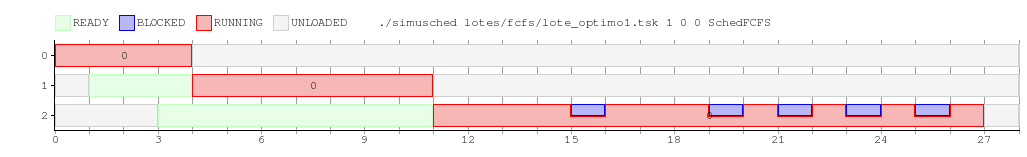
\includegraphics[scale=0.6]{FCFS/optimo1.png}
% \caption{Ejemplo donde $FCFS$ es óptimo.}
% \end{figure}
% 
% \begin{figure}[!H]
% 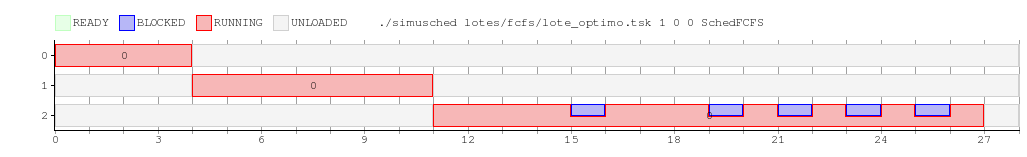
\includegraphics[scale=0.6]{FCFS/optimo2.png}
% \caption{Ejemplo donde $FCFS$ es óptimo y el $TAT$ coincide con el tiempo de procesamiento}
% \end{figure}


\subsubsection{Response time}

Otra métrica conocida es la del $Response$ $time$ o tiempo de respuesta, que se define como el tiempo que tarda una tarea en devolver datos después de una llamada bloqueante para acceder a recursos de entrada y salida. Esta medida también es conocida como latencia e impacta directamente sobre la experiencia del usuario. Una latencia elevada da la impresión al usuario de que el sistema anda lento o se cuelga. Es una métrica principalmente aplicable a las tareas interactivas, ya que realizan varias de estas llamadas.
